\documentclass{standalone}
\usepackage{tikz}
\usepackage{ctex,siunitx,upgreek}
\setCJKmainfont{Noto Serif CJK SC}
\usepackage{tkz-euclide}
\usepackage{amsmath}
\usetikzlibrary{patterns, calc,3d}
\usetikzlibrary {decorations.pathmorphing,decorations.pathreplacing,decorations.shapes}
\begin{document}
\small
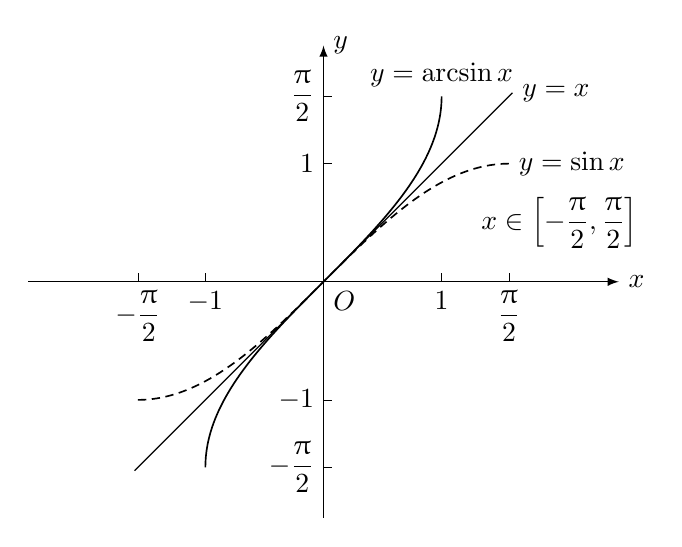
\begin{tikzpicture}[>=latex,scale=1.5]
  \draw[->](-2.5,0)--(2.5,0)node[right]{$x$};
  \draw[->](0,-2)--(0,2)node[right]{$y$};
  \node at (0,0)[below right]{$O$};
  \draw[semithick,samples=200,domain=-0.5*pi:0.5*pi] plot ({sin(\x r)},\x)node[above]{$y=\arcsin x$};
  \draw[semithick,densely dashed,samples=200,domain=-0.5*pi:0.5*pi] plot (\x,{sin(\x r)})node[right]{$y=\sin x$};
  \draw(-1.6,-1.6)--(1.6,1.6)node[right]{$y=x$};
  \foreach \x/\t in {1/1,0.5*pi/\dfrac\uppi2}
  {
    \draw[very thin](\x,0)node[below]{$\t$}--++(0,0.07);
    \draw[very thin](-\x,0)node[below]{$-\t$}--++(0,0.07);
    \draw[very thin](0,\x)node[left]{$\t$}--++(0.07,0);
    \draw[very thin](0,-\x)node[left]{$-\t$}--++(0.07,0);
  }
  \node at (2.0,0.2)[above]{$x\in\left[-\dfrac\uppi2,\dfrac\uppi2\right]$};
\end{tikzpicture}
\end{document}